\documentclass[11pt]{article}

% ACL Rolling Review / NAACL template. "review": anonymous with line numbers (submission);
% "preprint": non-anonymous with page numbers; "final": camera-ready.
\usepackage[preprint]{acl}

\usepackage{times}
\usepackage{latexsym}
\usepackage[T1]{fontenc}
\usepackage[utf8]{inputenc}
\usepackage{microtype}
\usepackage{inconsolata}
\usepackage{graphicx}
\usepackage{booktabs}
\usepackage{amsmath}
\usepackage{amsfonts}
\usepackage{array}
\usepackage{tabularx}
\usepackage{placeins}
\usepackage{float}
\usepackage{xcolor}
\newcolumntype{P}[1]{>{\raggedright\arraybackslash}p{#1}}
\newcolumntype{Y}{>{\raggedright\arraybackslash}X}
\makeatletter\setlength{\@fptop}{0pt}\setlength{\@dblfptop}{0pt}\makeatother   % top-align float pages (appendix tables)

\newcommand{\method}{Gauss6\slash FullVA}
\IfFileExists{stats.tex}{\newcommand{\nHuman}{39}
\newcommand{\nTurns}{2\,025}
\newcommand{\nTools}{1\,308}
\newcommand{\nEntries}{66}
\newcommand{\nHarness}{25}
\newcommand{\nShell}{2}
}{}
\providecommand{\nHuman}{36}\providecommand{\nTurns}{1\,700}\providecommand{\nTools}{1\,100}
\providecommand{\nEntries}{63}\providecommand{\nHarness}{25}\providecommand{\nShell}{2}

\title{Agentic auto-research in numerical analysis:\\
a coding agent finds, proves and validates\\
a sixth-order Lie-group integrator}

\author{Jingquan Wang \\
  Department of Mechanical Engineering \\
  University of Wisconsin--Madison \\
  \texttt{jingquanw@wisc.edu}}

\begin{document}
\maketitle

\begin{abstract}
We report a research program in computational mechanics carried out by a large-language-model
coding agent under human direction, from the first prototype to a manuscript with machine-checked
proofs, and analyse what made the outcome trustworthy and where it nearly was not. Over four months
the agent produced 49 versioned experiments on Lie-group integrators for constrained multibody
systems, converged on a three-stage Gauss collocation step with full velocity- and
acceleration-level constraint enforcement, and then discovered, while auditing its own manuscript
against its own code, that the implemented stage system is exactly reduced Gauss collocation lifted
to absolute coordinates. That identity became the central theorem of the resulting paper; the agent
formalized it in Lean~4 (57 theorems), designed and ran the experiments, and wrote the manuscript.
The process is the subject of this paper: a versioned exploration tree, an evidence ledger of 183
validators that pin every claim to an artefact, a proof sandbox, persistent cross-session memory,
explicit command boundaries, and a manuscript pipeline that checks every table entry against its
result file. We document ten incidents in which a wrong claim was caught and by what: four by
validators or purpose-built experiments, four by the agent's own cross-checks, two only by the human
reading the output. The human typed \nHuman{} messages in the final session against \nTools{} agent tool calls; the messages that mattered were judgments of taste, scope and fairness
rather than instructions. We release the repository, the ledger and the transcript.
\end{abstract}

\section{Introduction}
\label{sec:intro}

Coding agents built on large language models can now read a code base, run experiments, edit
proofs and write prose for days at a time. Whether they can carry a research program is a
different question, and the evidence so far comes mostly from short, benchmark-shaped tasks: an
idea to test, a paper to replicate, a Kaggle competition to enter
\citep{lu2024aiscientist,chan2025mlebench,starace2025paperbench}. Real research is longer, its
success criteria move, and its characteristic failure is not a crash but a claim that is slightly
stronger than what was shown. In numerical analysis this failure mode is acute: a convergence plot
can look sixth order for the wrong reason, a comparison with a public code can be unfair in ways
that take a domain expert to see, and a theorem can be true of a slightly different method than
the one implemented.

This paper is a longitudinal case study of one such program, conducted between May and September
2026 by LLM coding agents under the direction of a single human researcher. The subject of the
program was a high-order time integrator for constrained multibody systems modelled in absolute
coordinates on a Lie group. Its outcome is a method, \method{}, with an exact algebraic identity at
its core, a sixth-order error theorem whose algebra and perturbation lemmas are machine-checked in
Lean~4, and a numerical study on a frictional chain and on the four public ASME benchmark
mechanisms; that result is reported in a companion manuscript \citep{wang2026gauss6} and
summarized for a general reader in Figure~\ref{fig:problem}. Here we
report on the process: what the agent did, how the work was organized so that its claims could be
trusted, what went wrong, what caught it, and what the human actually contributed.

We make four contributions. (1)~\textbf{A documented instance} of agentic research with a
non-trivial result: the 49 versioned experiments, the 341 ledger scripts, the Lean development,
the manuscript and the transcript of the final phase are released, so the process can be inspected
rather than described. (2)~\textbf{A process architecture} (Section~\ref{sec:system}) of six
components that kept the program honest, from a versioned exploration tree to a manuscript
pipeline whose validator checks every printed number against its result file.
(3)~\textbf{A trajectory analysis} (Section~\ref{sec:trajectory}) of how the method emerged:
which hypotheses were rejected and why, and how an audit of the manuscript against the code
produced the central theorem. (4)~\textbf{An incident analysis} (Section~\ref{sec:incidents}) of
ten wrong or misleading claims, classified by what detected them: validators and purpose-built
experiments caught four, the agent's own cross-checks four, and the human two, both by looking at
a page or a figure and saying that it looked wrong.

Our reading of the evidence is that the agent was reliable at what can be checked mechanically and
unreliable at what cannot, and that the design consequence is not to keep the human in every loop
but to build loops that end in an artefact a machine can check, routing the few residual
judgments to the human.

\section{Related work}
\label{sec:related}

\paragraph{Automated scientific discovery with LLM agents}
End-to-end systems generate ideas, run experiments and write papers
\citep{lu2024aiscientist,yamada2025aiscientistv2,schmidgall2025agentlab,jansen2025codescientist},
propose hypotheses for wet-lab science \citep{gottweis2025coscientist}, or drive laboratory
automation \citep{boiko2023coscientist,bran2024chemcrow}. Their evaluations are many short projects judged by
reviewers or a rubric; the systems are the object of study and the science is the test bed. We
invert this: one research program is the object, the science is real (a method that did not exist
before, with a proof), and the question is what process made its claims hold up. Program-search systems such as FunSearch and AlphaEvolve
\citep{romeraparedes2024funsearch,novikov2025alphaevolve} discover objects that an automatic
evaluator scores; our setting has no scalar score, and the evaluators (validators, proofs,
convergence orders) had to be built as part of the work. Studies of LLM-generated research ideas
\citep{si2025ideas} stop at the idea stage; our concern is the long tail after it.

\paragraph{Agents for software engineering and ML engineering}
Benchmarks such as SWE-bench, MLE-bench, MLAgentBench, ScienceAgentBench and PaperBench
\citep{jimenez2024swebench,chan2025mlebench,huang2024mlagentbench,chen2025scienceagentbench,starace2025paperbench}
measure agents on tasks with a known target and a fixed grader. The coding-agent interface we used
\citep{yang2024sweagent,anthropic2025claudecode} is the same kind of tool; here the target moved as
the program learned what was true, and the grader had to be constructed and later frozen when it
became stale (Section~\ref{sec:system}). Architectures that interleave reasoning and acting or
reflect on failures \citep{yao2023react,shinn2023reflexion} describe the inner loop; we describe
the outer scaffolding a months-long program needed around it.

\paragraph{Machine-checked mathematics}
Language models prove theorems in Lean and other systems
\citep{yang2023leandojo,song2024leancopilot,xin2024deepseekprover,jiang2023dsp,trinh2024alphageometry}.
Our use is different in kind: the agent used Lean~4 with Mathlib \citep{demoura2021lean4,mathlib2020}
as an instrument to check its own analysis of its own code, transcribing the implemented residual
into Lean and proving that a specific 132-row system vanishes at a specific point. The
formalization did not produce the mathematics; it produced the confidence that the informal
argument, written by the same agent, had no gap.

\section{The research problem and its outcome}
\label{sec:problem}

\begin{figure*}[t]
  \centering
  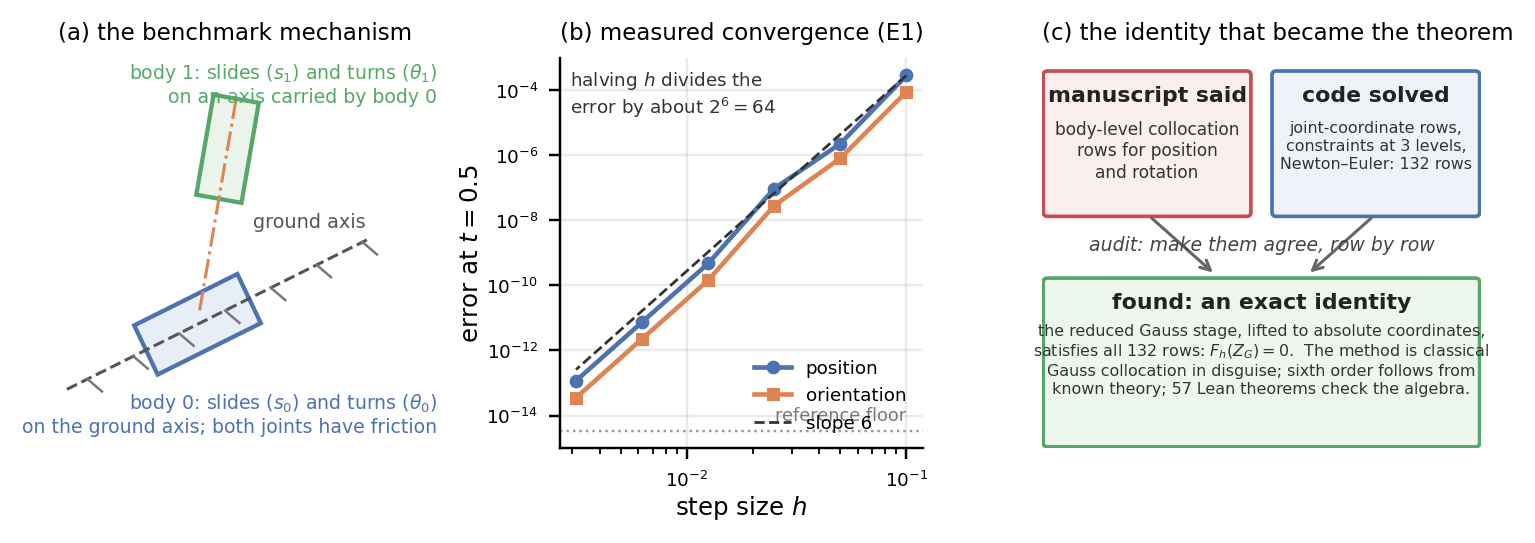
\includegraphics[width=\textwidth]{figures/fig_problem.png}
  \caption{The research problem and what came out of it. (a)~The benchmark: two rigid bodies, each
  sliding and turning on an axis, with friction in both joints. A time integrator advances all
  positions, rotations and velocities by a step $h$ while keeping the joints exactly closed.
  (b)~The measured error of the final method on this benchmark at $t=0.5$, from the E1 result file:
  the slope of $6$ on log axes is what ``sixth order'' means. (c)~The central result. Auditing the
  manuscript against the code showed that the two described different equations; making them
  agree revealed that the implemented stage system is satisfied exactly by the classical Gauss
  collocation solution, which is why the order is six.}
  \label{fig:problem}
\end{figure*}

\paragraph{Problem, in plain terms}
A mechanism is a set of rigid bodies connected by joints (Figure~\ref{fig:problem}a). Simulating it
means advancing every body's position and rotation through time in small steps $h$. The
difficulty is that the joints impose algebraic constraints: at every instant the bodies must
remain connected, their velocities must be compatible with staying connected, and so must their
accelerations. Standard time integrators satisfy such constraints only approximately, and the
approximation drifts. Rotations add a second difficulty, since they live on a curved space
(the Lie group $SO(3)$), not in a vector space. Joint friction adds a third. The accuracy of an
integrator is summarized by its \emph{order} $p$: halving the step divides the error by $2^p$.
Methods for this class that keep rotations on the group were of order two, or were designed for
unconstrained problems; a recent method reaches higher order on pendulum problems
\citep{chaturvedi2026tfe}; the companion manuscript reviews the literature
\citep{munthekaas1998rk,bruls2012lie,hairer1996solving,kissel2022absolute,fang2023halfimplicit}. The program set out to find a method of order higher than four, with a
proof of its order, for the full constrained problem with friction.

\paragraph{Outcome}
The method, \method{}, advances the mechanism by solving one nonlinear system per step. Its
unknowns are the positions, rotations, velocities, accelerations and joint forces at three
intermediate ``stage'' times (132 numbers for the benchmark); its equations are the constraints at
all three levels, the equations of motion at each stage, and Gauss collocation conditions on the
joint coordinates. Its measured order is six (Figure~\ref{fig:problem}b). The central theoretical
result (Figure~\ref{fig:problem}c) is that this 132-row system is solved exactly by a much older
object: the Gauss collocation solution of the mechanism's equations written in \emph{joint}
coordinates, once that solution is expressed in the body coordinates the method uses. The method is
therefore classical Gauss collocation in disguise, and its sixth order follows from a known theorem
rather than from a new estimate; the two things the implementation adds (a velocity-level closure
at the end of the step and an inexact nonlinear solve) are perturbations of size $h^7$ with
explicit constants. The identity, the perturbation chain and the properties of the Gauss tableau
are proved in Lean~4 (57 theorems). Numerically the method is sixth order on the chain of
Figure~\ref{fig:problem}a and on a public double-pendulum benchmark, and reaches errors below
$10^{-10}$ where the public reference codes for this problem class have errors of order one
\citep{wang2026gauss6}.

\paragraph{Why this is a good test of agentic research}
None of this is a benchmark score. It required choosing among method families, building verifiers
that did not exist, recognizing that a coding convention was an identity, formalizing it, designing
experiments with defensible references and error measures, and writing for a journal audience.
Each is a place where an agent can produce something that looks right and is not, and
Section~\ref{sec:incidents} shows that it did.

\section{The process architecture}
\label{sec:system}

\begin{figure*}[t]
  \centering
  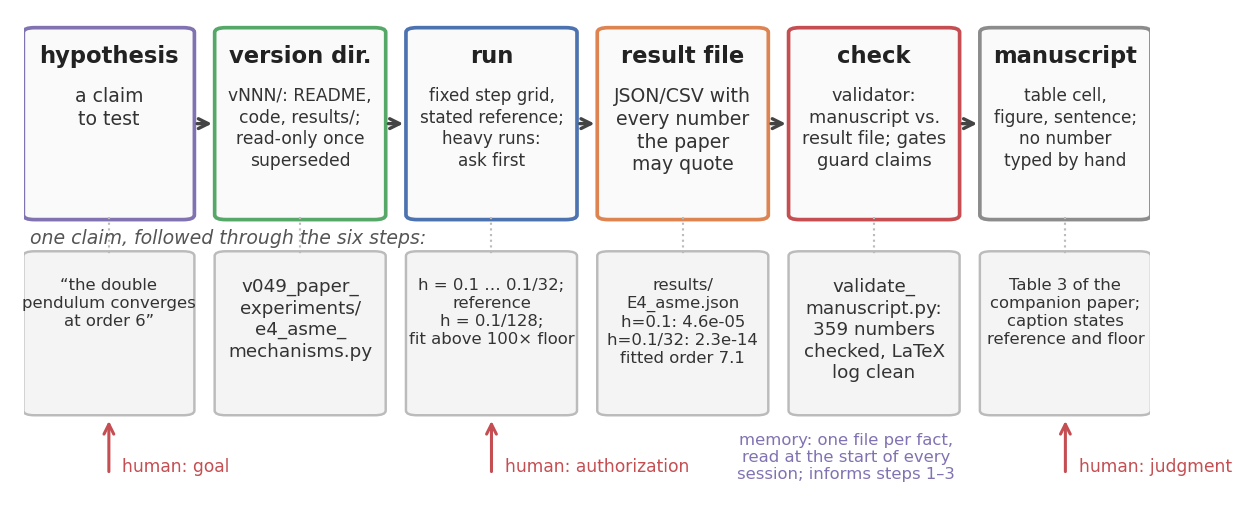
\includegraphics[width=\textwidth]{figures/fig_process.png}
  \caption{The process, and one claim followed through it. Top row: the six steps every claim
  passes through. Bottom row: the claim ``the double pendulum converges at order 6'' as it
  actually travelled: a script in a versioned directory, a run with a stated reference solution
  and a stated floor below which no order is fitted, a result file holding the numbers, a
  validator that checks each printed number against that file, and the table cell in the companion
  paper. The human enters at three points; memory carries facts between sessions; the external
  campaign runs only on explicit authorization.}
  \label{fig:process}
\end{figure*}

The agent was a general-purpose coding agent \citep{anthropic2025claudecode} with file, shell,
LaTeX, Lean and git access, working in a repository on the researcher's machine. Nothing in the
agent was specialized to the domain. What was specialized is the set of artefacts the agent had to
produce and consult, which Figure~\ref{fig:process} lays out as the path a single claim takes. We
describe the six components and, for each, the failure it was introduced to prevent.

\paragraph{Versioned exploration tree}
Every hypothesis about the method got its own directory \texttt{vNNN\_<name>} with a README, the
scripts and a \texttt{results/} folder; once superseded it became read-only and new work started a
new version. Forty-nine exist (Figure~\ref{fig:tree}a). The rule prevents the most common way an
agent loses information: editing a working script in place until the earlier state, and the reason
it was abandoned, are gone. It also makes negative results first-class: the Lobatto node swap
(v024), the projection repair (v025), matrix-free Newton--Krylov (v032) and Jacobian lagging
(v033) are preserved with the numbers that ruled them out (Figure~\ref{fig:tree}b), and the
manuscript cites them as things that were tried.

\paragraph{Evidence ledger: builders, validators, gates}
The ledger separates producing evidence from checking it. \emph{Builders} (146 scripts) read
result files and write JSON and Markdown records: convergence tables, constraint norms, Newton
statistics, claim inventories. \emph{Validators} (183 scripts) read those records and the
manuscript and assert relations between them: a quoted order equals the recorded fit, a forbidden
phrase is absent, a cited file exists with the recorded hash, a gate's preconditions hold. The
top-level validator ran $4\,896$ checks and the paper-package validator $162\,327$. \emph{Gates}
are named preconditions for stronger claims (the exact-identity gate, for instance, requires the
Lean copy in the repository to be byte-identical to the development and its axiom audit clean).
The failure this prevents is claim drift: a diagnostic row becoming a result, a consistency check becoming a proof, a number in
the text outliving the run that produced it. The ledger has a cost: by September it pinned
hundreds of phrases of a 13\,000-line manuscript and had shaped it into an audit report. When the
manuscript was rewritten (Section~\ref{sec:trajectory}) the ledger was \emph{frozen}, pointed at a
snapshot of the old paper as the historical record, and replaced for the new paper by the one
validator of the last step below.

\paragraph{Proof sandbox}
The analysis lives in a Lean~4/Mathlib project outside the working tree, with a copy in the
repository that a gate keeps synchronized. Fifty-seven theorems cover the row identities of the
implemented residual (transcribed into Lean), the perturbation lemmas with explicit constants, the
quadrature bound, the order conditions of the Gauss tableau and the local-to-global transfer. A
check script builds the project and runs an exhaustive axiom audit; two classical theorems enter as
cited results, and this is stated. The sandbox changed the paper: formalizing the theorem's
hypotheses showed that two of them follow from smoothness, and those derivations became lemmas.

\paragraph{Persistent memory}
The agent's context is finite and sessions end. A memory directory holds one file per fact, with a
one-line description and a type, and an index loaded at the start of every session. Eleven such
files exist; they record, for example, that the benchmark leaves its regular branch at
$t\approx0.6$ and all chain experiments therefore stop at $T=0.5$ (Figure~\ref{fig:incidents}b),
and that the human judged the earlier manuscript poor. The failure this prevents is repetition: an
agent that has learned why an experiment fails would otherwise run it again next session.

\paragraph{Command and authorization boundaries}
Some commands are expensive or change the meaning of the evidence. The pipeline contract lists
them: the full campaign of the method implementation is never run as a routine check, default
$h=10^{-4}$ reruns are forbidden, and the external ``source-policy'' campaign against the public
codes runs only on explicit human authorization; its driver refuses to start unless a literal
approval sentence is passed to it. The one time it ran (September~20) the human's instruction was
two words (``run B4''); the agent supplied the sentence, recorded that it had done so, and the
campaign executed 13 commands and promoted 0 of 40 rows, with the reason written down. The
boundary is procedural rather than technical, since the agent can type the sentence; what it buys
is a deliberate, recorded step.

\paragraph{Manuscript pipeline}
\label{sec:manuscript}
The rewritten manuscript is assembled from section files by a script and its figures are drawn
from result files by another, so no number is typed; a validator checks that the LaTeX log is
clean, that every number in every result table equals a value in the result file the table cites
(359 checks), that every Lean theorem named in the paper exists, and that the arXiv and flat copies
were generated from the current source. This prevents what the old ledger prevented with phrase
pins, at a fraction of the cost and without shaping the prose.

\section{Trajectory: how the method was found}
\label{sec:trajectory}

\begin{figure*}[t]
  \centering
  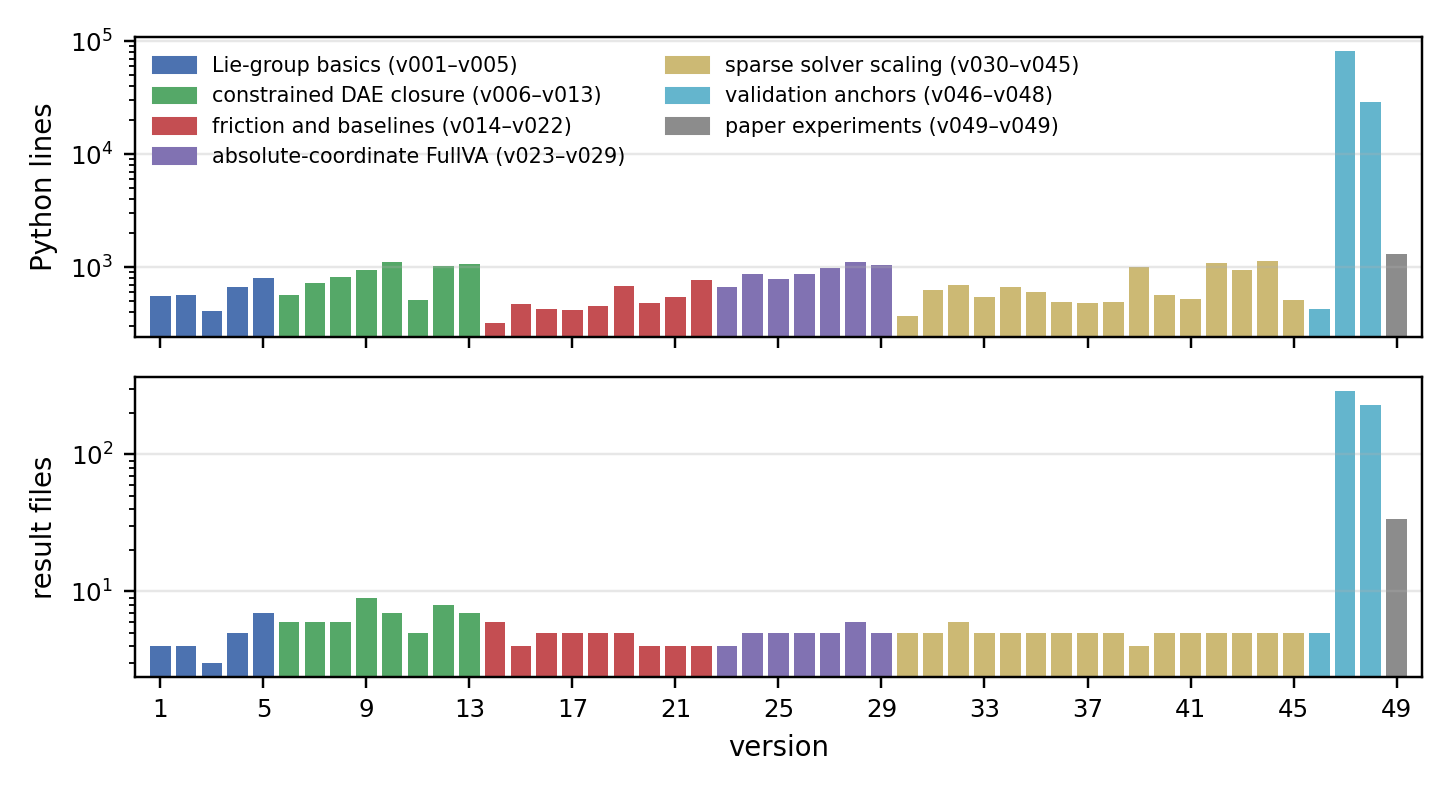
\includegraphics[width=0.92\textwidth]{figures/fig_versions.png}
  \caption{The 49 versioned experiments, coloured by phase, with the size of their code and the
  number of result files each left behind. The exploratory burst v001--v048 was produced in about three weeks in late May and early June 2026;
  v046--v048 (validation anchors) and v049 (paper experiments) carry the bulk of the artefacts.}
  \label{fig:versions}
\end{figure*}

Appendix~\ref{app:ledger} condenses the exploration into phases (Table~\ref{tab:phases}) and lists
every version (Table~\ref{tab:ledger}). In outline: Lie-group basics and the choice of Gauss
collocation (v001--v005); constrained DAE closure in absolute coordinates, friction, automatic
differentiation and quaternions (v006--v013); friction regimes and the rejection of trapezoidal, BDF
and Lobatto baselines (v014--v022); the absolute-coordinate revolute DAE and the emergence of the
FullVA stage system (v023--v029); sixteen versions of sparse-solver work (v030--v045); validation
anchors (v046--v048); and the experiments of the rewritten paper (v049). Three features of the
trajectory matter for the argument of this paper.


\paragraph{Negative results were the steering signal}
Of the 48 exploratory versions, about twenty exist to rule something out. The pattern that produced the
method is v023--v029: a full absolute-coordinate revolute DAE (v023) showed endpoint
velocity-level constraint drift; swapping Gauss nodes for Lobatto (v024) did not remove it;
projecting the endpoint after the step (v025) removed it but changed the method; adding the
velocity-level constraint rows at the stages (v026) and then the acceleration-level rows (v027)
removed it without changing the method. The last of these is the FullVA stage system. Its
generalization to a second joint (v029) and to non-revolute pairs (v043--v044) then tested that
the construction was not specific to one mechanism. Without the preserved negative results the
same agent, in a later session, would have retried the projection repair; the memory of why it was
wrong is what the versioned tree stores.

\paragraph{Sixteen versions of solver work produced no paper result, and that is recorded}
v030--v045 investigated sparse Jacobians for the growing stage systems. The sparse structure was
found, coloured and cached correctly, and dense automatic differentiation remained faster on every
problem tried. The ledger records ``sparse structure verified'' and forbids ``sparse speed
superiority''; the companion paper says one sentence about it. An agent optimizing for a paper
would have dropped or dressed up this phase; the ledger made the honest outcome the cheap one.

\paragraph{The theorem came from an audit, not from a search}
By September the manuscript displayed the stage system as body-level collocation rows, while the
code solved joint-coordinate collocation rows together with the full constraint hierarchy. The
agent was asked to reconcile the two. Working through the row inventory it found that the
$132$-row residual is zero at the lifted reduced Gauss stage, that the converse holds on the
regular branch, and hence that the implemented method \emph{is} reduced Gauss collocation in
disguise. This replaced what had been a conditional order argument with an open stage-residual
hypothesis by an exact identity plus two explicit perturbations, and it made the sixth order a
consequence of classical theory rather than a conjecture supported by slopes. The Lean development
was started the same day to check the identity row by row; the two hypotheses that the earlier
argument had kept as assumptions were then derived from smoothness. The discovery was not the
agent proposing a new idea. It was the agent being required to make two descriptions of the same
object agree, and refusing to paper over the difference.

\paragraph{The rewrite}
The manuscript that the ledger had grown around was 13\,000 lines, then 4\,000 after a
compaction, and read as a catalogue of what was not claimed. The human judged it poor. The agent
proposed a full rewrite with a new experiment set, delivered an outline, an experiment plan with
costs and an introduction for review, and after approval executed it: seven experiments, three
schematic figures, a 44-page manuscript with its arXiv and flat copies, and the new validator, in
about four days with \nHuman{} human messages (Section~\ref{sec:quant}).

\section{Incidents: wrong claims and what caught them}
\label{sec:incidents}

We recorded every case during the final phase in which a statement that had been written or was
about to be written turned out to be wrong or misleading. Table~\ref{tab:incidents} lists them with
the mechanism that detected each. We group the mechanisms into three kinds: \emph{artefact
checks} (a validator or an experiment built to test the statement), \emph{agent cross-checks} (the
agent noticing an inconsistency between two things it had itself produced), and \emph{human
judgment} (the researcher looking at the output and objecting).

\begin{table}[!htbp]
\centering
\caption{Incidents in the final phase. ``Detected by'' is the mechanism that first raised the
problem; A = artefact check (validator or purpose-built experiment), C = agent cross-check, H =
human judgment.}
\label{tab:incidents}
\scriptsize
\begin{tabularx}{\linewidth}{@{}P{0.02\linewidth}P{0.27\linewidth}P{0.25\linewidth}P{0.15\linewidth}Y@{}}
\toprule
\# & Wrong or misleading statement & Cause & Detected by & Resolution \\
\midrule
1 & The manuscript was sound but unreadable: hundreds of ``diagnostic'', ``non-claim'' and
``boundary'' sentences. & Every validator-pinned phrase had been written to satisfy the pin. & H
(``the paper quality feels poor'') & Full rewrite; ledger frozen; one number-checking validator. \\
2 & Orientation error converged at order 2.2 while position, velocity and angular velocity
converged at order 6.2. & Geodesic angle computed as $2\arccos(p\cdot q)$, whose resolution floor
is $3\times10^{-8}$ rad. & C (one of four quantities disagreed) & Chord formula
$2\arcsin(\lVert p\mp q\rVert/2)$; orientation order 6.28. \\
3 & Reference runs on the chain failed at $h=0.1/256$ over $T=1$; the plan said $T=1$ and
$T=20$. & The benchmark's frozen sliding direction degenerates at $t\approx0.605$ ($n_1\cdot a_1\to0$),
a modelling limit, not a solver failure. & A (Newton residual $6\times10^{5}$) then H (chose to
keep the model and stop at $T=0.5$) & All chain experiments on $[0,0.5]$; limit stated in the
paper. \\
4 & Driven single pendulum: velocity error rose and fell erratically between $10^{-15}$ and
$4\times10^{-9}$ while position showed order 6. & The harness's Newton predictor is the analytic
solution and the stage Jacobian has condition number $10^{10}$--$10^{13}$; velocities carry
amplified roundoff. & H (``why does the top-left panel look strange?'') & Velocity not reported for
that mechanism; the panel labelled as a reconstruction check; mechanism explained. \\
5 & The four ASME mechanisms were planned as four convergence tests. & Three of the four are
kinematically driven; their motion is fixed by the drive. & A (errors at $10^{-14}$ for all $h$) &
Only the double pendulum is a dynamics test; the others are consistency rows. \\
6 & The public-code comparison at $T=3$ showed the public methods with $O(1)$ errors; suspicion of
a model mismatch. & The double pendulum amplifies perturbations over $T=3$. & C (added a $T=0.1$
alignment run: first-order decrease, same model) & Comparison kept with the alignment check
reported. \\
7 & ``The $h^7$-scaled stopping rule with $c_\eta=10^{4}$ covers the reported grids.'' & With the
fixed tolerance $10^{-11}$, the accepted residual over $h^7$ reaches $10^{6}$ at the finest
step. & A (purpose-built experiment E7) & Statement replaced by the measured ratios and a
discussion of the pessimistic bound. \\
8 & The single pendulum ``converges at order 6 with a floor'' was fitted over roundoff points,
giving 3.6. & Fit used a zero floor for the analytic reference. & C & Roundoff floor $10^{-15}$;
fit 6.0 over the resolved points. \\
9 & ``All results generated from a single implementation path.'' & Four harnesses assemble the
same stage system for four mechanisms. & C (self-review) & Reworded; assemblies listed. \\
10 & After the rewrite the frozen ledger reported stale line counts and lost markers. & Its
snapshot records pinned the sizes of scripts that had changed. & A (frozen validators) & Builder
sequence rerun; both frozen chains green. \\
\bottomrule
\end{tabularx}
\end{table}

\FloatBarrier
\paragraph{What the artefact checks caught}
Incidents 3, 5, 7 and 10 were caught by things that fail loudly: a Newton solve that does not
converge, a table full of $10^{-14}$, a purpose-built measurement, a validator. Incident~7 is the
instructive one. The analysis section stated that the fixed-tolerance runs satisfy the solver
hypothesis with a modest constant; the agent wrote an experiment (E7) whose only purpose was to
measure that constant, and the measurement contradicted the text by six orders of magnitude on the
finest grid. The text was rewritten to report the measurement. Where experiments are cheap and the
norm is to measure a claimed constant rather than argue for it, a class of overclaims becomes data.

\paragraph{What the agent's cross-checks caught}
Incidents 2, 6, 8 and 9 were caught because the agent had produced two things that had to agree
and did not: four error measures of which one behaved differently, a comparison whose magnitude
called for a sanity check at a shorter horizon, a fit whose value contradicted the visible slope,
and a sentence in the introduction that the methods section did not support. These are the same
habit that produced the central theorem (Section~\ref{sec:trajectory}): redundancy that the agent is
required to reconcile.

\paragraph{What only the human caught}
Incidents 1 and 4, and the decision in Incident 3, needed a person. Incident 1 is a judgment of
quality that no validator expressed and the agent did not have: the manuscript satisfied every check
and was bad. Incident 3 was a modelling decision (keep the benchmark as implemented and stop at
$T=0.5$, or change the joint model) that the agent escalated with three options and a
recommendation to change the model; the human chose to keep it, and the limit was documented.
Incident 4 is the one we find most important. The agent had seen the non-monotone velocity curve,
written a plausible and wrong explanation (a tolerance artefact of the harness), and moved on. The
human's objection was not technical (``it looks strange''). The investigation it triggered found
that the harness starts Newton at the exact solution and that the Jacobian is ill-conditioned by ten
to thirteen orders, a fact about the benchmark that no validator could have known to check. Looking
at figures is not a formality.

\section{Quantitative account}
\label{sec:quant}

\begin{figure*}[t]
  \centering
  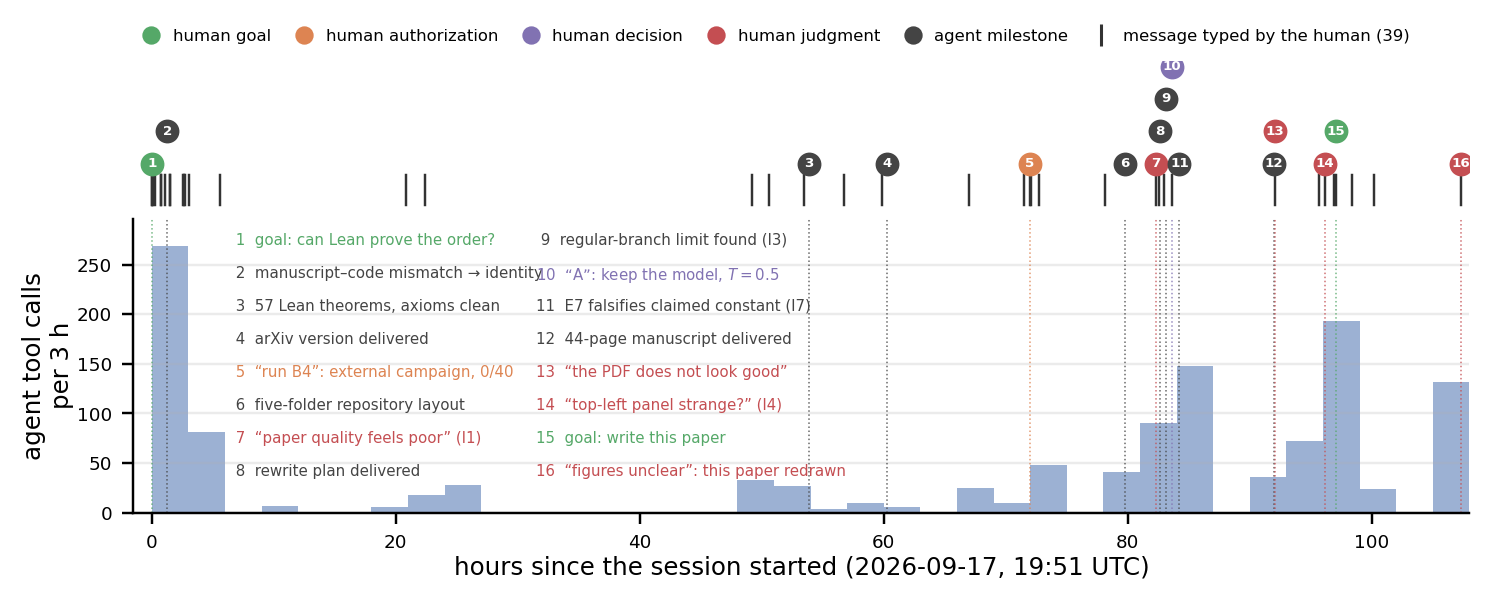
\includegraphics[width=\textwidth]{figures/fig_session.png}
  \caption{The final session, from its transcript. Bars: agent tool calls per three hours. Ticks in
  the strip: the \nHuman{} messages typed by the human. Numbered markers: milestones and the
  human's interventions, keyed in the empty region of the plot and coloured by kind. The identity
  was found within the first two hours (event~2); the rewrite (events 7--12) took about ten hours
  of agent time and four human messages; the two remaining human judgments (13, 14) and the
  request for this paper (15) came after the manuscript was delivered. The gaps are hours in which
  the human was away and the agent idle.}
  \label{fig:session}
\end{figure*}

\paragraph{Effort}
The program left 49 versioned experiments with 793 result files, 341 ledger scripts, 57 Lean
theorems, a 44-page manuscript and 11 memory files (Table~\ref{tab:artefacts},
Appendix~\ref{app:cost}). Figure~\ref{fig:session} profiles the final session, in which the Lean
development was built, the manuscript rewritten and this paper drafted: of its \nTools{} tool
calls about a third were validators and manuscript builds, a third inspection and editing of
files, a tenth Lean, and a twentieth experiments. Earlier phases were not recorded as transcripts
and are documented by the version ledger and the dated logs.

\paragraph{What the human said}
Of the transcript's \nEntries{} user-role entries, \nHarness{} are harness-generated and
\nShell{} are shell commands; \nHuman{} were typed by the human. They fall into six kinds (Appendix~\ref{app:messages}): goals (twelve), approvals of the agent's own proposals
(nine), authorizations (three), decisions (two), judgments (four) and questions (six); the rest
were acknowledgments. None contained a technical instruction about the method, the proofs or the
experiments. The judgments produced Incidents 1 and 4, the layout overhaul of the manuscript and
the redrawing of this paper's figures; the benchmark-horizon decision went against the agent's
recommendation.

\paragraph{What the agent did without being asked}
It chose the experiment set and its reference policy, found and fixed the orientation-angle
formula, discovered and escalated the regular-branch limit, added the alignment check for the
public comparison, wrote the experiment that falsified its own claim, froze the old ledger, and
wrote the memory files for the next session. It also produced the human-caught errors.

\section{Discussion}
\label{sec:discussion}

\paragraph{Where the agent was reliable, and where not}
It was reliable at everything that ended in an artefact a machine could check: the Lean
development has no gaps because Lean would not accept them, the tables match the result files
because a validator reads both, the negative results survived because the directory structure made
deleting them harder than keeping them. It was unreliable at everything that ended in a sentence.
Incident~1 is the clearest: a manuscript that passed $162\,327$ checks and was, in the researcher's
words, poor, because the prose had become a transcript of checks the agent had itself proposed. Incident~4 is the subtler one: the agent saw an anomaly, produced an
explanation of the right shape, and accepted it. Both are failures of judgment, invisible to every
mechanism except a person reading.

\paragraph{Design consequences}
Three follow. First, every claim should be routed toward an artefact check: if a constant is
asserted, write the experiment that measures it (Incident~7); if two descriptions of the same object
exist, require them to agree (the theorem). Second, validators should check facts, not prose: the
frozen ledger pinned phrases and shaped the paper; its replacement pins numbers to files. Third, the
human's attention should be spent on outputs, not process: the human-caught incidents came from
reading a page and looking at a figure, and none of the \nHuman{} messages needed expertise beyond
recognizing that something looked wrong.

\section{Conclusion}
\label{sec:conclusion}

A coding agent carried a research program from a prototype to a manuscript with
a new theorem, a machine-checked proof and a defensible numerical study. What made the outcome
trustworthy was not the agent's judgment but artefacts that turned judgments into checks:
versioned experiments that could not be edited away, a ledger tying claims to records, a proof
assistant that would not accept a gap, memory across sessions, boundaries on what could be run
unasked, and a manuscript whose numbers are read from files. The few residual judgments were the
human's; the practical question is not how to remove the human but how to arrange the work so that
those judgments land on the right pages.

\section*{Limitations}
This is a single case: one program, one domain, one researcher, one family of coding agents, and no
control condition. We cannot say how a different agent, the same agent without the scaffolding, or a
human-only effort of the same duration would have fared, and the counts in Table~\ref{tab:artefacts}
measure output, not quality. The transcript covers only the final phase; the four earlier months are
documented by the versioned tree, the dated ledger records and the git history, so the incident list
is complete for the final phase and reconstructed for the earlier ones, and incidents that left no
trace are invisible to us. The classification of the human messages (Appendix~\ref{app:messages}) was
made by the author and the agent from the paraphrased transcript; another reader might draw the
category boundaries differently, although the total is fixed. The scaffolding was designed and built
by the agent itself and is therefore only as good as the agent's idea of what to check; the frozen
ledger (Section~\ref{sec:system}) is direct evidence that this idea can drift, and the authorization
boundary is procedural rather than technical. Finally, the domain is one in which every claim has a
numerical or formal referee (a convergence order, a proof kernel); we do not know how much of the
architecture transfers to fields where the checkable artefact is harder to define.

\section*{Ethics Statement}
The agent chose the experiments, found the identity, wrote the proofs, ran the comparisons and wrote
the text of the companion manuscript, and it drafted this paper from the repository and the
transcript. The human set the goal, judged the result, made the one modelling decision that was
escalated, authorized network access, the GitHub push and one external campaign, and is responsible
for the content of both papers; the companion manuscript discloses the use of an AI coding
assistant. Under current norms the agent is a tool and the human is the author; the transcript
makes the division inspectable. No human subjects were involved, and the only personal data in the
released material are the author's own messages. The public codes compared against are used as
published under their licences, and the comparison is reported with its reference policy and horizon
so that it can be contested. We see two risks in work of this kind: that agentic research is
presented as more autonomous than it was, which is why the human's contribution is reported message
by message, and that checks written by the agent are mistaken for independent review, of which
Incident~1 is our own example.


\bibliography{references}

\appendix
\raggedbottom
\renewcommand{\dbltopfraction}{0.95}\renewcommand{\dblfloatpagefraction}{0.85}\setcounter{dbltopnumber}{3}
\section{The 49 versions}
\label{app:ledger}

\begin{table*}[t]
\centering
\small
\begin{tabularx}{\textwidth}{P{0.12\linewidth}P{0.22\linewidth}YY}
\toprule
Versions & Phase & Kept & Ruled out \\
\midrule
v001--v005 & Lie-group basics: $SO(3)$ benchmarks, corrected right-action CF4/RKMK4, Yoshida
composition, two-stage Gauss--Lie & Gauss collocation as the high-order family; right-action
conventions & Yoshida composition (negative substeps unsuitable for friction) \\
v006--v013 & Constrained DAE closure: reduced fixed-pivot DAE, absolute-coordinate Gauss DAE,
endpoint constraints inside Newton, friction, AD Jacobian, quaternion transport, three-stage Gauss
& absolute coordinates; endpoint constraints in the solve; JAX automatic differentiation;
quaternions; six stages & position-only closure; finite-difference Jacobians \\
v014--v022 & Friction regimes and baselines: smoothness sweep, adaptive Gauss6/4, trapezoidal,
BDF2 and Lobatto baselines, multiplier-dependent Brown--McPhee friction & Brown--McPhee law through
the multipliers; the smooth/sharp split as a stated regime & trapezoidal, BDF2 and Lobatto endpoint
methods as accuracy candidates; adaptivity as the main result \\
v023--v029 & Absolute-coordinate revolute DAE: full DAE, Lobatto node swap, projection repair,
stage velocity rows, stage acceleration rows, off-axis torque, two joints & \emph{stage-level
velocity and acceleration constraint rows} (``FullVA''), the decisive move & node swap; post-step
projection as a fix \\
v030--v045 & Sparse solver scaling: Jacobian sparsity, sparse Newton, matrix-free Krylov, lagging,
coloured AD, symbolic patterns, caches, larger topologies, prismatic joints & correctness of
sparse patterns; prismatic and skew-axis coverage & every speed claim: dense AD stayed faster \\
v046--v048 & Validation anchors: four ASME mechanisms, two-body cylindrical chain pipeline,
cross-paper benchmark harness & the chain as the main benchmark; the public suite as the external
one & external superiority claims (source-policy rows 0/40) \\
v049 & Experiments for the rewritten paper & E1--E7 & long horizons ($T=1$, $T=20$) on the chain \\
\bottomrule
\end{tabularx}
\caption{Phases of the exploration. ``Kept'' is what survived into the final method; ``ruled out''
is preserved as a versioned negative result.}
\label{tab:phases}
\end{table*}

Table~\ref{tab:phases} condenses the exploration into phases; Table~\ref{tab:ledger} gives one line per version: the method family tested and the role the
version plays in the record (its ``current role'' field in the machine-readable ledger).

\begin{table*}[t]
\centering
\scriptsize\setlength{\tabcolsep}{3pt}
\begin{tabular}[t]{@{}p{0.025\textwidth}p{0.19\textwidth}p{0.245\textwidth}@{}}
\toprule
v & Method family & Role in the record \\
\midrule
001 & $SO(3)$ kinematics and Euler top & benchmark infrastructure \\
002 & CF4 and RKMK4 (right action) & prescribed-orientation baseline, order four \\
003 & public rA code reproduction & reproducibility anchor for the public suite \\
004 & Yoshida-composed Lie midpoint & conservative baseline; negative substeps unsuitable for friction \\
005 & two-stage Gauss--Lie & smooth conservative mechanics, order four \\
006 & reduced fixed-pivot Gauss DAE & reduced constrained prototype \\
007 & absolute-coordinate Gauss DAE & index-3 consistency lesson \\
008 & endpoint-constrained Gauss DAE & projection-free absolute-coordinate prototype \\
009 & frictional endpoint Gauss4 & friction order-reduction evidence \\
010 & JAX AD Jacobian & nonlinear-solve backend \\
011 & $S^3$ transport operators & bridge to the quaternion formulation \\
012 & quaternion endpoint Gauss4 & verified quaternion residual \\
013 & Gauss6 endpoint collocation & first smooth sixth-order candidate \\
014 & Gauss4 vs Gauss6 friction sweep & smoothness decision rule \\
015 & adaptive embedded Gauss6/4 & near-nonsmooth regime tool \\
016 & reduced Lie-trapezoidal & ruled out as accuracy candidate \\
017 & reduced Lie-BDF2 & ruled out as accuracy candidate \\
018 & reduced Lie-Lobatto endpoint & TFE-style baseline ruled out \\
019 & multiplier-dependent Stribeck friction & AD-friendly friction through multipliers \\
020 & adaptive multiplier friction & sharp-friction regime tool \\
021 & Brown--McPhee multiplier friction & the friction law kept \\
022 & revolute Brown--McPhee Gauss6/4 & paper-like revolute friction evidence \\
023 & absolute-coordinate revolute Gauss DAE & full DAE; endpoint drift exposed \\
024 & direct Lobatto full revolute DAE & node swap ruled out \\
025 & projected absolute revolute DAE & projection repair: works, changes the method \\
\bottomrule
\end{tabular}\hfill
\begin{tabular}[t]{@{}p{0.025\textwidth}p{0.19\textwidth}p{0.245\textwidth}@{}}
\toprule
v & Method family & Role in the record \\
\midrule
026 & stage pivot-velocity rows & non-projection closure, velocity level \\
027 & stage velocity + acceleration rows & \textbf{FullVA}: the stage system kept \\
028 & off-axis FullVA revolute & axis-torque stress test \\
029 & double-revolute FullVA & generalizes to two joints \\
030 & Jacobian sparsity diagnosis & motivates sparse solvers \\
031 & sparse Newton & correct; not faster \\
032 & matrix-free Newton--Krylov & ruled out \\
033 & lagged sparse Newton & ruled out \\
034 & coloured-JVP sparse Jacobian & correct structured sparse AD \\
035 & batched coloured JVP & sparse-AD backend \\
036 & block-symbolic sparse pattern & production-style pattern \\
037 & JVP-pruned pattern & pattern discovery \\
038 & pattern cache reuse & cache policy \\
039 & triple-revolute scaling & transfer to larger topology \\
040 & generated block triple pattern & pattern acquisition \\
041 & triple-revolute cache refresh & cache policy \\
042 & skew-axis triple revolute & non-coplanar geometry \\
043 & skew prismatic pair & first non-revolute pair \\
044 & double-prismatic chain & interbody prismatic pair \\
045 & row-coloured VJP sparse AD & sparse-assembly diagnostic \\
046 & four ASME mechanisms & public-suite validation anchor \\
047 & two-body cylindrical chain pipeline & the main benchmark and the accepted implementation \\
048 & cross-paper same-test harness & external comparison scaffold; 0/40 source-policy rows \\
049 & paper experiments E1--E7 & the numerical section of the rewritten manuscript \\
\bottomrule
\end{tabular}
\caption{Version ledger (condensed from \texttt{validation/docs/version\_ledger.csv}).}
\label{tab:ledger}
\end{table*}

\section{Memory files}
\label{app:memory}

The eleven memory files at the end of the program, by their one-line descriptions: where the Lean
project lives and why it is kept off the synchronized drive; what the Lean development covers and
what it must not be claimed to close; the row-family mismatch between manuscript and code and its
resolution ($F(Z_G)=0$ exactly); the manuscript compaction of September~17 and the builder order;
the implemented predictor's zero angular guesses and their consequence for the Newton lemma; the
derived arXiv version and how it is rebuilt; the five-folder repository layout and its path
routing; the guarded external campaign of September~20 (approval sentence, 0/40 rows, why it
cannot close by execution); the paper rewrite of September~20--21 and its state; the benchmark's
regular-branch limit and the choice $T=0.5$; and the driven single-pendulum harness whose predictor
is the analytic drive. Each file has a ``why'' and a ``how to apply'' paragraph; the index is
loaded at the start of every session.

\section{Human messages of the final session}
\label{app:messages}

The \nHuman{} messages typed by the human (the other \nHarness{} user-role entries of the
transcript are harness-generated: task notifications, command echoes, compaction summaries and
image attachments; \nShell{} more are shell commands typed for the GitHub login), lightly
paraphrased from Chinese and grouped. \emph{Goals} (12): can Lean prove the convergence order;
install it; run the Lean check and report; continue and look for problems; tidy the Lean
development; make an arXiv version in a simple template; reorganize the folders; split the LaTeX
out of the ledger; make a clean five-folder layout keeping only the best manuscript; read it again
and find what else is wrong; write this paper; keep fixing. \emph{Approvals of the agent's own
proposals} (9): ``do as you said'' and variants, including the two approvals of the rewrite plan.
\emph{Authorizations} (3): any permission including network access; push to GitHub as you see fit;
run the external campaign. \emph{Decisions} (2): option A for the benchmark horizon, against the
agent's recommendation; target NAACL rather than a machine-learning conference for this paper.
\emph{Judgments} (4): the paper quality feels poor; the PDF does not look good, visualize the
pages; why does the top-left panel of Figure~7 look strange; this paper's quality is very poor,
the figures and the content are unclear. \emph{Questions} (6): what is this doing; what do you
think is appropriate; what does that mean; what is still missing; what is the status; what else is
there to do. \emph{Other} (3): an acknowledgment, ``continue'', and a report that the GitHub login
had failed.

\section{The incidents in full}
\label{app:incidents}

Table~\ref{tab:incidents_full} gives, for each incident of Table~\ref{tab:incidents}, the
wrong statement, its cause, the detector and the resolution.

\begin{table*}[t]
\centering
\scriptsize
\begin{tabularx}{\textwidth}{@{}P{0.02\linewidth}P{0.27\linewidth}P{0.25\linewidth}P{0.15\linewidth}Y@{}}
\toprule
\# & Wrong or misleading statement & Cause & Detected by & Resolution \\
\midrule
1 & The manuscript was sound but unreadable: hundreds of ``diagnostic'', ``non-claim'' and
``boundary'' sentences. & Every validator-pinned phrase had been written to satisfy the pin. & H
(``the paper quality feels poor'') & Full rewrite; ledger frozen; one number-checking validator. \\
2 & Orientation error converged at order 2.2 while position, velocity and angular velocity
converged at order 6.2. & Geodesic angle computed as $2\arccos(p\cdot q)$, whose resolution floor
is $3\times10^{-8}$ rad. & C (one of four quantities disagreed) & Chord formula
$2\arcsin(\lVert p\mp q\rVert/2)$; orientation order 6.28. \\
3 & Reference runs on the chain failed at $h=0.1/256$ over $T=1$; the plan said $T=1$ and
$T=20$. & The benchmark's frozen sliding direction degenerates at $t\approx0.6$,
a modelling limit, not a solver failure. & A (Newton residual $6\times10^{5}$) then H (chose to
keep the model and stop at $T=0.5$) & All chain experiments on $[0,0.5]$; limit stated in the
paper. \\
4 & Driven single pendulum: velocity error rose and fell erratically between $10^{-15}$ and
$4\times10^{-9}$ while position showed order 6. & The harness's Newton predictor is the analytic
solution and the stage Jacobian has condition number $10^{10}$--$10^{13}$; velocities carry
amplified roundoff. & H (``why does the top-left panel look strange?'') & Velocity not reported for
that mechanism; the panel labelled as a reconstruction check; mechanism explained. \\
5 & The four ASME mechanisms were planned as four convergence tests. & Three of the four are
kinematically driven; their motion is fixed by the drive. & A (errors at $10^{-14}$ for all $h$) &
Only the double pendulum is a dynamics test; the others are consistency rows. \\
6 & The public-code comparison at $T=3$ showed the public methods with $O(1)$ errors; suspicion of
a model mismatch. & The double pendulum amplifies perturbations over $T=3$. & C (added a $T=0.1$
alignment run: first-order decrease, same model) & Comparison kept with the alignment check
reported. \\
7 & ``The $h^7$-scaled stopping rule with $c_\eta=10^{4}$ covers the reported grids.'' & With the
fixed tolerance $10^{-11}$, the accepted residual over $h^7$ reaches $10^{6}$ at the finest
step. & A (purpose-built experiment E7) & Statement replaced by the measured ratios and a
discussion of the pessimistic bound. \\
8 & The single pendulum ``converges at order 6 with a floor'' was fitted over roundoff points,
giving 3.6. & Fit used a zero floor for the analytic reference. & C & Roundoff floor $10^{-15}$;
fit 6.0 over the resolved points. \\
9 & ``All results generated from a single implementation path.'' & Four harnesses assemble the
same stage system for four mechanisms. & C (self-review) & Reworded; assemblies listed. \\
10 & After the rewrite the frozen ledger reported stale line counts and lost markers. & Its
snapshot records pinned the sizes of scripts that had changed. & A (frozen validators) & Builder
sequence rerun; both frozen chains green. \\
\bottomrule
\end{tabularx}
\caption{The ten incidents of the final phase in full (Table~\ref{tab:incidents} of the main text is the condensed version). ``Detected by'' is the mechanism that first raised the
problem; A = artefact check (validator or purpose-built experiment), C = agent cross-check, H =
human judgment.}
\label{tab:incidents_full}
\end{table*}

\section{Artefacts and cost of the checks}
\label{app:cost}

\begin{table}[H]
\centering
\small
\begin{tabular}{@{}lr@{}}
\toprule
Versioned experiments & 49 \\
Result files & 793 \\
Python lines (all) & 356\,167 \\
Lean files / lines / theorems & 10 / 1\,672 / 57 \\
Manuscript & 44 pp., 51 refs \\
Ledger scripts (builders / validators) & 341 (146 / 183) \\
Ledger records (JSON / Markdown) & 171 / 186 \\
Ledger checks (top-level / package) & 4\,896 / 162\,327 \\
Manuscript validator checks & 359 \\
Memory files & 11 \\
\bottomrule
\end{tabular}
\caption{What the program produced (repository state at the end of the final phase).}
\label{tab:artefacts}
\end{table}

The frozen ledger's two validation chains take about twenty minutes, the builder sequence that
refreshes their snapshots ten, the new manuscript validator two seconds, and the Lean check under a
minute once the Mathlib cache is present. The longest single computation was the $h=10^{-4}$
double-pendulum reference over $T=3$ (1.6~h), computed once and cached.


\end{document}
